\section{Identificação e extração do elemento máximo}

\begin{frame}[fragile]{Identificação e extração do elemento máximo}

    \begin{itemize}
        \item O elemento máximo de uma \textit{max heap} está localizado na raiz da árvore

        \item Portanto a identificação deste elemento pode ser feita em $O(1)$

        \item A extração deste elemento é o processo reverso da inserção

        \item A raiz deve ser substituída pela folha mais à direita do último nível

        \item Esta substituição pode gerar uma violação da propriedade fundamentação do
            nó em relação aos seus filhos

        \item As possíveis violações devem ser resolvidas da raiz para as folhas

        \item Se a violação ocorrem com ambos filhos, deve-se escolher o que possui a 
            maior informação para prosseguir com as trocas

        \item Esta extração tem complexidade $O(\log N)$
    \end{itemize}

\end{frame}

\begin{frame}[fragile]{Exemplo de extração em uma \textit{heap} binária} 

    \begin{figure}
        \centering
        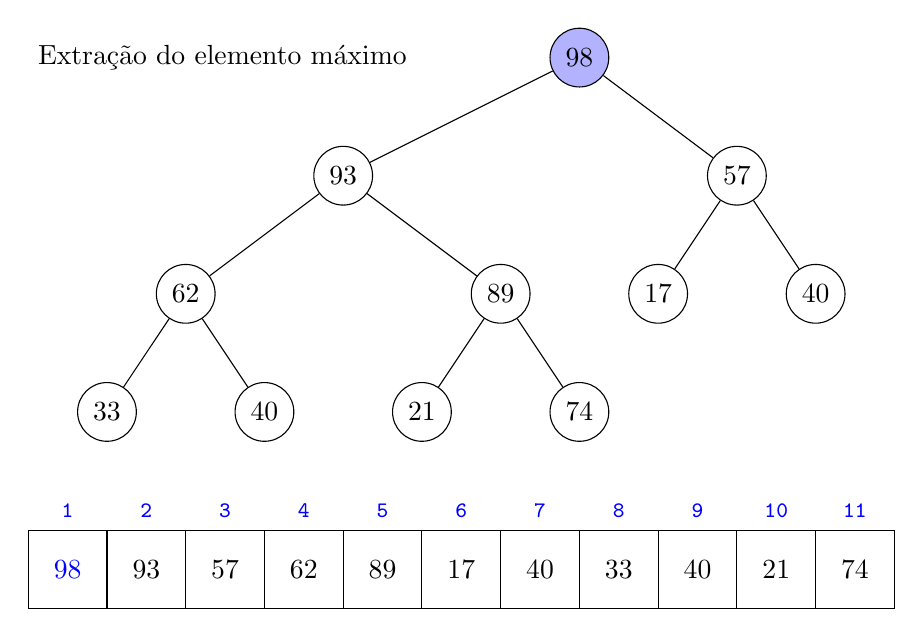
\begin{tikzpicture}
                \node[anchor=west] at (-1, 6) { Extração do elemento máximo };
                \node[circle,draw,fill=blue!30] (A) at (6, 6) { 98 };
                \node[circle,draw] (B) at (3, 4.5) { \textcolor{black}{93} };
                \node[circle,draw] (C) at (8, 4.5) { 57 };
                \node[circle,draw] (D) at (1, 3) { 62 };
                \node[circle,draw] (E) at (5, 3) { 89 };
                \node[circle,draw] (F) at (7, 3) { 17 };
                \node[circle,draw] (G) at (9, 3) { 40 };
                \node[circle,draw] (H) at (0, 1.5) { 33 };
                \node[circle,draw] (I) at (2, 1.5) { 40 };
                \node[circle,draw] (J) at (4, 1.5) { 21 };
                \node[circle,draw] (K) at (6, 1.5) { 74 };

                \draw (A) -- (B);
                \draw (A) -- (C);
                \draw (B) -- (D);
                \draw (B) -- (E);
                \draw (C) -- (F);
                \draw (C) -- (G);
                \draw (D) -- (H);
                \draw (D) -- (I);
                \draw (E) -- (J);
                \draw (E) -- (K);

                \draw (-1, -1) grid (10, 0);

                \node[color=blue] at (-0.5, 0.25) { \footnotesize \texttt{\textbf{1}} };
                \node[color=blue] at (0.5, 0.25) { \footnotesize \texttt{\textbf{2}} };
                \node[color=blue] at (1.5, 0.25) { \footnotesize \texttt{\textbf{3}} };
                \node[color=blue] at (2.5, 0.25) { \footnotesize \texttt{\textbf{4}} };
                \node[color=blue] at (3.5, 0.25) { \footnotesize \texttt{\textbf{5}} };
                \node[color=blue] at (4.5, 0.25) { \footnotesize \texttt{\textbf{6}} };
                \node[color=blue] at (5.5, 0.25) { \footnotesize \texttt{\textbf{7}} };
                \node[color=blue] at (6.5, 0.25) { \footnotesize \texttt{\textbf{8}} };
                \node[color=blue] at (7.5, 0.25) { \footnotesize \texttt{\textbf{9}} };
                \node[color=blue] at (8.5, 0.25) { \footnotesize \texttt{\textbf{10}} };
                \node[color=blue] at (9.5, 0.25) { \footnotesize \texttt{\textbf{11}} };

                \node at (-0.5, -0.5) { \textcolor{blue}{98} };
                \node at (0.5, -0.5) { \textcolor{black}{93} };
                \node at (1.5, -0.5) { 57 };
                \node at (2.5, -0.5) { 62 };
                \node at (3.5, -0.5) { \textcolor{black}{89} };
                \node at (4.5, -0.5) { 17 };
                \node at (5.5, -0.5) { 40 };
                \node at (6.5, -0.5) { 33 };
                \node at (7.5, -0.5) { 40 };
                \node at (8.5, -0.5) { 21 };
                \node at (9.5, -0.5) { \textcolor{black}{74} };
        \end{tikzpicture}
    \end{figure}

\end{frame}

\begin{frame}[fragile]{Exemplo de extração em uma \textit{heap} binária} 

    \begin{figure}
        \centering
        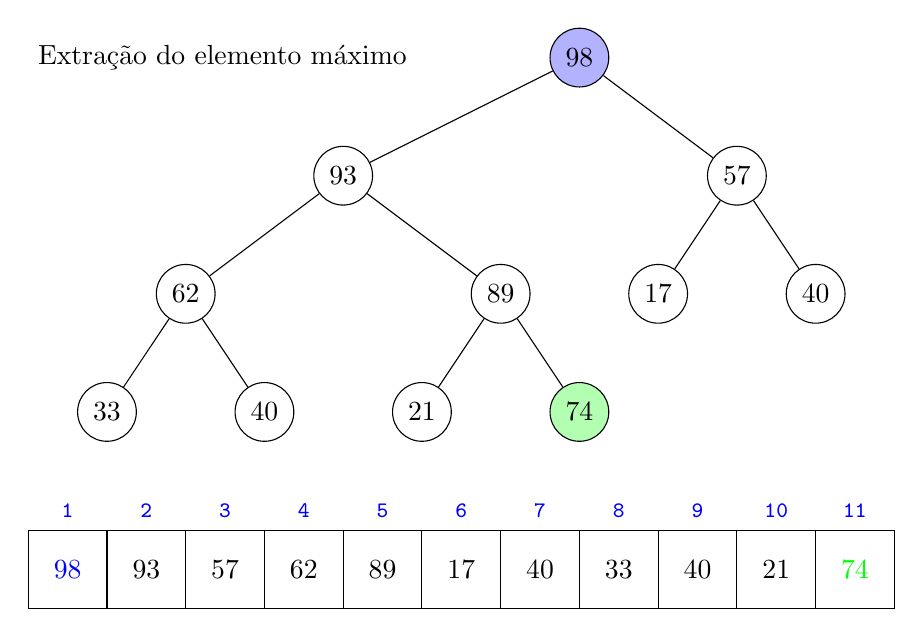
\begin{tikzpicture}
                \node[anchor=west] at (-1, 6) { Extração do elemento máximo };
                \node[circle,draw,fill=blue!30] (A) at (6, 6) { 98 };
                \node[circle,draw] (B) at (3, 4.5) { \textcolor{black}{93} };
                \node[circle,draw] (C) at (8, 4.5) { 57 };
                \node[circle,draw] (D) at (1, 3) { 62 };
                \node[circle,draw] (E) at (5, 3) { 89 };
                \node[circle,draw] (F) at (7, 3) { 17 };
                \node[circle,draw] (G) at (9, 3) { 40 };
                \node[circle,draw] (H) at (0, 1.5) { 33 };
                \node[circle,draw] (I) at (2, 1.5) { 40 };
                \node[circle,draw] (J) at (4, 1.5) { 21 };
                \node[circle,draw,fill=green!30] (K) at (6, 1.5) { 74 };

                \draw (A) -- (B);
                \draw (A) -- (C);
                \draw (B) -- (D);
                \draw (B) -- (E);
                \draw (C) -- (F);
                \draw (C) -- (G);
                \draw (D) -- (H);
                \draw (D) -- (I);
                \draw (E) -- (J);
                \draw (E) -- (K);

                \draw (-1, -1) grid (10, 0);

                \node[color=blue] at (-0.5, 0.25) { \footnotesize \texttt{\textbf{1}} };
                \node[color=blue] at (0.5, 0.25) { \footnotesize \texttt{\textbf{2}} };
                \node[color=blue] at (1.5, 0.25) { \footnotesize \texttt{\textbf{3}} };
                \node[color=blue] at (2.5, 0.25) { \footnotesize \texttt{\textbf{4}} };
                \node[color=blue] at (3.5, 0.25) { \footnotesize \texttt{\textbf{5}} };
                \node[color=blue] at (4.5, 0.25) { \footnotesize \texttt{\textbf{6}} };
                \node[color=blue] at (5.5, 0.25) { \footnotesize \texttt{\textbf{7}} };
                \node[color=blue] at (6.5, 0.25) { \footnotesize \texttt{\textbf{8}} };
                \node[color=blue] at (7.5, 0.25) { \footnotesize \texttt{\textbf{9}} };
                \node[color=blue] at (8.5, 0.25) { \footnotesize \texttt{\textbf{10}} };
                \node[color=blue] at (9.5, 0.25) { \footnotesize \texttt{\textbf{11}} };

                \node at (-0.5, -0.5) { \textcolor{blue}{98} };
                \node at (0.5, -0.5) { \textcolor{black}{93} };
                \node at (1.5, -0.5) { 57 };
                \node at (2.5, -0.5) { 62 };
                \node at (3.5, -0.5) { \textcolor{black}{89} };
                \node at (4.5, -0.5) { 17 };
                \node at (5.5, -0.5) { 40 };
                \node at (6.5, -0.5) { 33 };
                \node at (7.5, -0.5) { 40 };
                \node at (8.5, -0.5) { 21 };
                \node at (9.5, -0.5) { \textcolor{green}{74} };
        \end{tikzpicture}
    \end{figure}

\end{frame}

\begin{frame}[fragile]{Exemplo de extração em uma \textit{heap} binária} 

    \begin{figure}
        \centering
        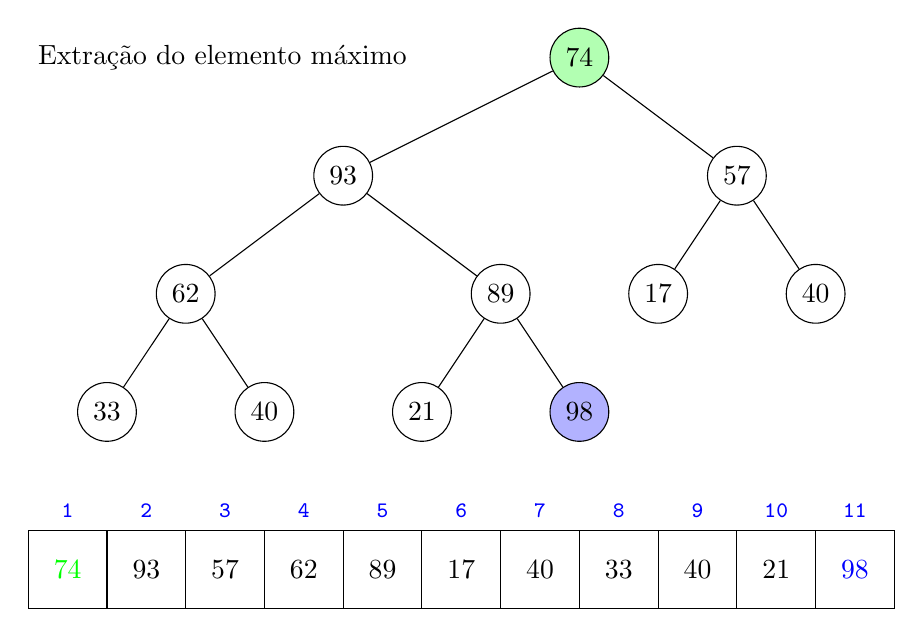
\begin{tikzpicture}
                \node[anchor=west] at (-1, 6) { Extração do elemento máximo };
                \node[circle,draw,fill=green!30] (A) at (6, 6) { 74 };
                \node[circle,draw] (B) at (3, 4.5) { \textcolor{black}{93} };
                \node[circle,draw] (C) at (8, 4.5) { 57 };
                \node[circle,draw] (D) at (1, 3) { 62 };
                \node[circle,draw] (E) at (5, 3) { 89 };
                \node[circle,draw] (F) at (7, 3) { 17 };
                \node[circle,draw] (G) at (9, 3) { 40 };
                \node[circle,draw] (H) at (0, 1.5) { 33 };
                \node[circle,draw] (I) at (2, 1.5) { 40 };
                \node[circle,draw] (J) at (4, 1.5) { 21 };
                \node[circle,draw,fill=blue!30] (K) at (6, 1.5) { 98 };

                \draw (A) -- (B);
                \draw (A) -- (C);
                \draw (B) -- (D);
                \draw (B) -- (E);
                \draw (C) -- (F);
                \draw (C) -- (G);
                \draw (D) -- (H);
                \draw (D) -- (I);
                \draw (E) -- (J);
                \draw (E) -- (K);

                \draw (-1, -1) grid (10, 0);

                \node[color=blue] at (-0.5, 0.25) { \footnotesize \texttt{\textbf{1}} };
                \node[color=blue] at (0.5, 0.25) { \footnotesize \texttt{\textbf{2}} };
                \node[color=blue] at (1.5, 0.25) { \footnotesize \texttt{\textbf{3}} };
                \node[color=blue] at (2.5, 0.25) { \footnotesize \texttt{\textbf{4}} };
                \node[color=blue] at (3.5, 0.25) { \footnotesize \texttt{\textbf{5}} };
                \node[color=blue] at (4.5, 0.25) { \footnotesize \texttt{\textbf{6}} };
                \node[color=blue] at (5.5, 0.25) { \footnotesize \texttt{\textbf{7}} };
                \node[color=blue] at (6.5, 0.25) { \footnotesize \texttt{\textbf{8}} };
                \node[color=blue] at (7.5, 0.25) { \footnotesize \texttt{\textbf{9}} };
                \node[color=blue] at (8.5, 0.25) { \footnotesize \texttt{\textbf{10}} };
                \node[color=blue] at (9.5, 0.25) { \footnotesize \texttt{\textbf{11}} };

                \node at (-0.5, -0.5) { \textcolor{green}{74} };
                \node at (0.5, -0.5) { \textcolor{black}{93} };
                \node at (1.5, -0.5) { 57 };
                \node at (2.5, -0.5) { 62 };
                \node at (3.5, -0.5) { \textcolor{black}{89} };
                \node at (4.5, -0.5) { 17 };
                \node at (5.5, -0.5) { 40 };
                \node at (6.5, -0.5) { 33 };
                \node at (7.5, -0.5) { 40 };
                \node at (8.5, -0.5) { 21 };
                \node at (9.5, -0.5) { \textcolor{blue}{98} };
        \end{tikzpicture}
    \end{figure}

\end{frame}

\begin{frame}[fragile]{Exemplo de extração em uma \textit{heap} binária} 

    \begin{figure}
        \centering
        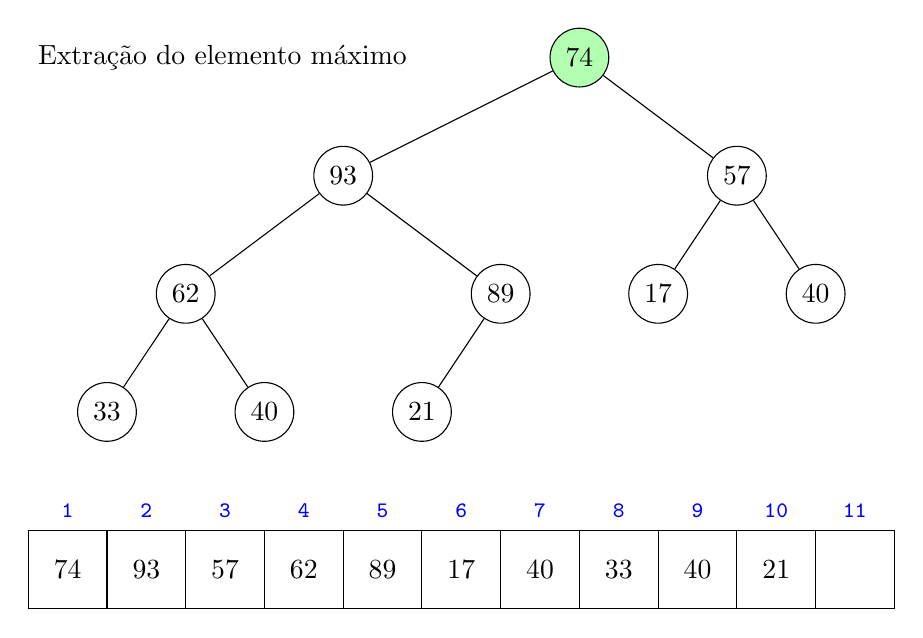
\begin{tikzpicture}
                \node[anchor=west] at (-1, 6) { Extração do elemento máximo };
                \node[circle,draw,fill=green!30] (A) at (6, 6) { 74 };
                \node[circle,draw] (B) at (3, 4.5) { \textcolor{black}{93} };
                \node[circle,draw] (C) at (8, 4.5) { 57 };
                \node[circle,draw] (D) at (1, 3) { 62 };
                \node[circle,draw] (E) at (5, 3) { 89 };
                \node[circle,draw] (F) at (7, 3) { 17 };
                \node[circle,draw] (G) at (9, 3) { 40 };
                \node[circle,draw] (H) at (0, 1.5) { 33 };
                \node[circle,draw] (I) at (2, 1.5) { 40 };
                \node[circle,draw] (J) at (4, 1.5) { 21 };

                \draw (A) -- (B);
                \draw (A) -- (C);
                \draw (B) -- (D);
                \draw (B) -- (E);
                \draw (C) -- (F);
                \draw (C) -- (G);
                \draw (D) -- (H);
                \draw (D) -- (I);
                \draw (E) -- (J);

                \draw (-1, -1) grid (10, 0);

                \node[color=blue] at (-0.5, 0.25) { \footnotesize \texttt{\textbf{1}} };
                \node[color=blue] at (0.5, 0.25) { \footnotesize \texttt{\textbf{2}} };
                \node[color=blue] at (1.5, 0.25) { \footnotesize \texttt{\textbf{3}} };
                \node[color=blue] at (2.5, 0.25) { \footnotesize \texttt{\textbf{4}} };
                \node[color=blue] at (3.5, 0.25) { \footnotesize \texttt{\textbf{5}} };
                \node[color=blue] at (4.5, 0.25) { \footnotesize \texttt{\textbf{6}} };
                \node[color=blue] at (5.5, 0.25) { \footnotesize \texttt{\textbf{7}} };
                \node[color=blue] at (6.5, 0.25) { \footnotesize \texttt{\textbf{8}} };
                \node[color=blue] at (7.5, 0.25) { \footnotesize \texttt{\textbf{9}} };
                \node[color=blue] at (8.5, 0.25) { \footnotesize \texttt{\textbf{10}} };
                \node[color=blue] at (9.5, 0.25) { \footnotesize \texttt{\textbf{11}} };

                \node at (-0.5, -0.5) { \textcolor{black}{74} };
                \node at (0.5, -0.5) { \textcolor{black}{93} };
                \node at (1.5, -0.5) { 57 };
                \node at (2.5, -0.5) { 62 };
                \node at (3.5, -0.5) { \textcolor{black}{89} };
                \node at (4.5, -0.5) { 17 };
                \node at (5.5, -0.5) { 40 };
                \node at (6.5, -0.5) { 33 };
                \node at (7.5, -0.5) { 40 };
                \node at (8.5, -0.5) { 21 };
        \end{tikzpicture}
    \end{figure}

\end{frame}

\begin{frame}[fragile]{Exemplo de extração em uma \textit{heap} binária} 

    \begin{figure}
        \centering
        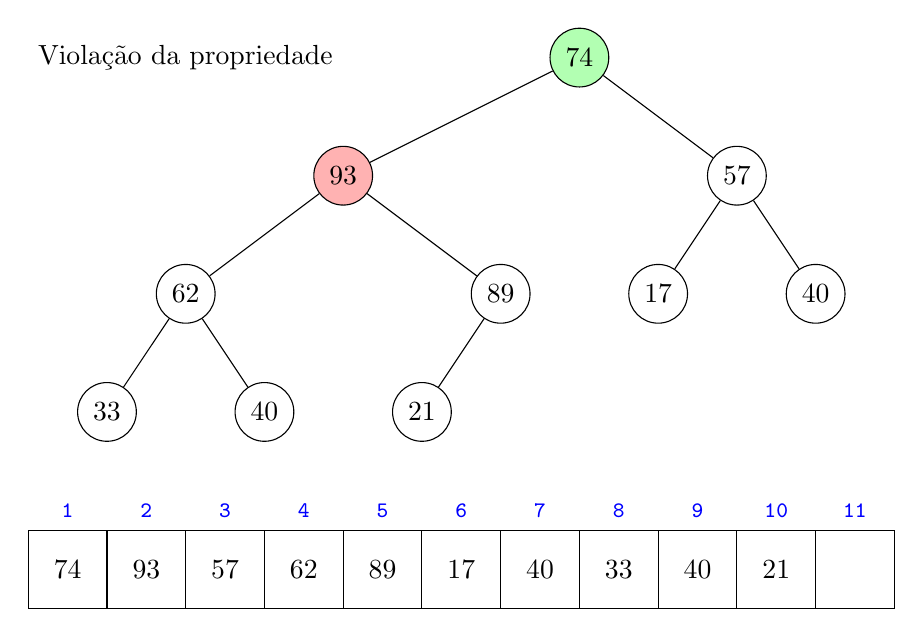
\begin{tikzpicture}
                \node[anchor=west] at (-1, 6) { Violação da propriedade };
                \node[circle,draw,fill=green!30] (A) at (6, 6) { 74 };
                \node[circle,draw,fill=red!30] (B) at (3, 4.5) { \textcolor{black}{93} };
                \node[circle,draw] (C) at (8, 4.5) { 57 };
                \node[circle,draw] (D) at (1, 3) { 62 };
                \node[circle,draw] (E) at (5, 3) { 89 };
                \node[circle,draw] (F) at (7, 3) { 17 };
                \node[circle,draw] (G) at (9, 3) { 40 };
                \node[circle,draw] (H) at (0, 1.5) { 33 };
                \node[circle,draw] (I) at (2, 1.5) { 40 };
                \node[circle,draw] (J) at (4, 1.5) { 21 };

                \draw (A) -- (B);
                \draw (A) -- (C);
                \draw (B) -- (D);
                \draw (B) -- (E);
                \draw (C) -- (F);
                \draw (C) -- (G);
                \draw (D) -- (H);
                \draw (D) -- (I);
                \draw (E) -- (J);

                \draw (-1, -1) grid (10, 0);

                \node[color=blue] at (-0.5, 0.25) { \footnotesize \texttt{\textbf{1}} };
                \node[color=blue] at (0.5, 0.25) { \footnotesize \texttt{\textbf{2}} };
                \node[color=blue] at (1.5, 0.25) { \footnotesize \texttt{\textbf{3}} };
                \node[color=blue] at (2.5, 0.25) { \footnotesize \texttt{\textbf{4}} };
                \node[color=blue] at (3.5, 0.25) { \footnotesize \texttt{\textbf{5}} };
                \node[color=blue] at (4.5, 0.25) { \footnotesize \texttt{\textbf{6}} };
                \node[color=blue] at (5.5, 0.25) { \footnotesize \texttt{\textbf{7}} };
                \node[color=blue] at (6.5, 0.25) { \footnotesize \texttt{\textbf{8}} };
                \node[color=blue] at (7.5, 0.25) { \footnotesize \texttt{\textbf{9}} };
                \node[color=blue] at (8.5, 0.25) { \footnotesize \texttt{\textbf{10}} };
                \node[color=blue] at (9.5, 0.25) { \footnotesize \texttt{\textbf{11}} };

                \node at (-0.5, -0.5) { \textcolor{black}{74} };
                \node at (0.5, -0.5) { \textcolor{black}{93} };
                \node at (1.5, -0.5) { 57 };
                \node at (2.5, -0.5) { 62 };
                \node at (3.5, -0.5) { \textcolor{black}{89} };
                \node at (4.5, -0.5) { 17 };
                \node at (5.5, -0.5) { 40 };
                \node at (6.5, -0.5) { 33 };
                \node at (7.5, -0.5) { 40 };
                \node at (8.5, -0.5) { 21 };
        \end{tikzpicture}
    \end{figure}

\end{frame}

\begin{frame}[fragile]{Exemplo de extração em uma \textit{heap} binária} 

    \begin{figure}
        \centering
        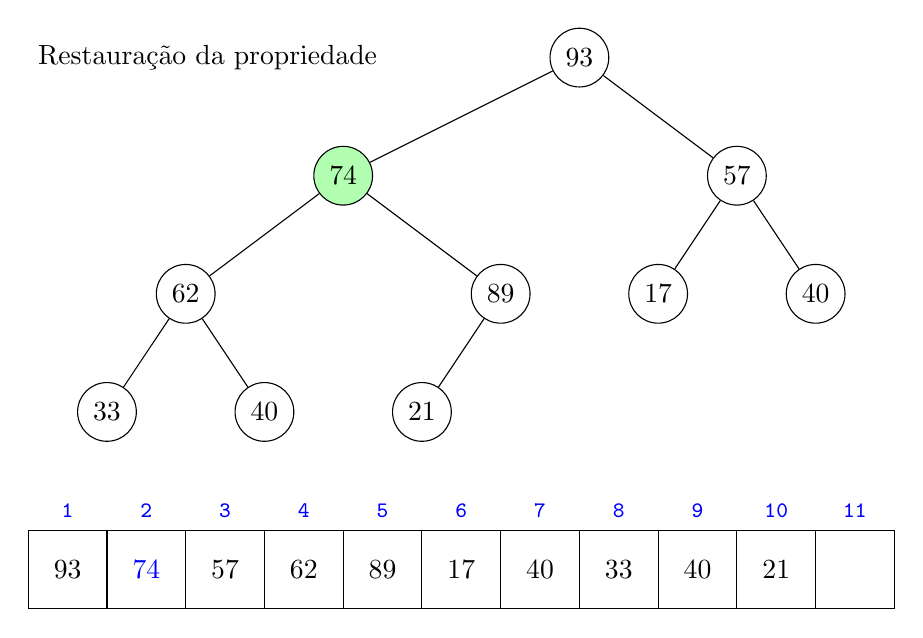
\begin{tikzpicture}
                \node[anchor=west] at (-1, 6) { Restauração da propriedade };
                \node[circle,draw] (A) at (6, 6) { 93 };
                \node[circle,draw,fill=green!30] (B) at (3, 4.5) { \textcolor{black}{74} };
                \node[circle,draw] (C) at (8, 4.5) { 57 };
                \node[circle,draw] (D) at (1, 3) { 62 };
                \node[circle,draw] (E) at (5, 3) { 89 };
                \node[circle,draw] (F) at (7, 3) { 17 };
                \node[circle,draw] (G) at (9, 3) { 40 };
                \node[circle,draw] (H) at (0, 1.5) { 33 };
                \node[circle,draw] (I) at (2, 1.5) { 40 };
                \node[circle,draw] (J) at (4, 1.5) { 21 };

                \draw (A) -- (B);
                \draw (A) -- (C);
                \draw (B) -- (D);
                \draw (B) -- (E);
                \draw (C) -- (F);
                \draw (C) -- (G);
                \draw (D) -- (H);
                \draw (D) -- (I);
                \draw (E) -- (J);

                \draw (-1, -1) grid (10, 0);

                \node[color=blue] at (-0.5, 0.25) { \footnotesize \texttt{\textbf{1}} };
                \node[color=blue] at (0.5, 0.25) { \footnotesize \texttt{\textbf{2}} };
                \node[color=blue] at (1.5, 0.25) { \footnotesize \texttt{\textbf{3}} };
                \node[color=blue] at (2.5, 0.25) { \footnotesize \texttt{\textbf{4}} };
                \node[color=blue] at (3.5, 0.25) { \footnotesize \texttt{\textbf{5}} };
                \node[color=blue] at (4.5, 0.25) { \footnotesize \texttt{\textbf{6}} };
                \node[color=blue] at (5.5, 0.25) { \footnotesize \texttt{\textbf{7}} };
                \node[color=blue] at (6.5, 0.25) { \footnotesize \texttt{\textbf{8}} };
                \node[color=blue] at (7.5, 0.25) { \footnotesize \texttt{\textbf{9}} };
                \node[color=blue] at (8.5, 0.25) { \footnotesize \texttt{\textbf{10}} };
                \node[color=blue] at (9.5, 0.25) { \footnotesize \texttt{\textbf{11}} };

                \node at (-0.5, -0.5) { \textcolor{black}{93} };
                \node at (0.5, -0.5) { \textcolor{blue}{74} };
                \node at (1.5, -0.5) { 57 };
                \node at (2.5, -0.5) { 62 };
                \node at (3.5, -0.5) { \textcolor{black}{89} };
                \node at (4.5, -0.5) { 17 };
                \node at (5.5, -0.5) { 40 };
                \node at (6.5, -0.5) { 33 };
                \node at (7.5, -0.5) { 40 };
                \node at (8.5, -0.5) { 21 };
        \end{tikzpicture}
    \end{figure}

\end{frame}

\begin{frame}[fragile]{Exemplo de extração em uma \textit{heap} binária} 

    \begin{figure}
        \centering
        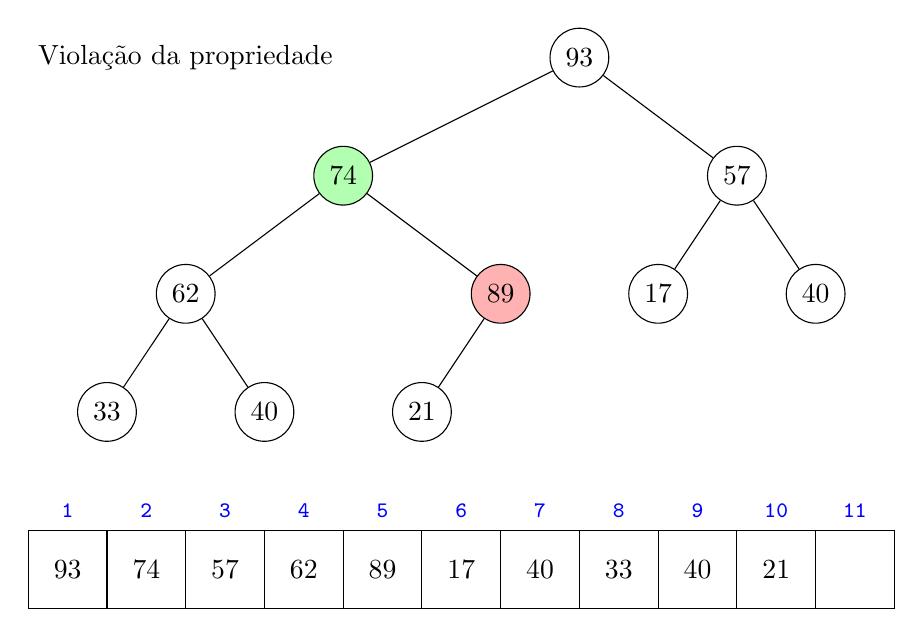
\begin{tikzpicture}
                \node[anchor=west] at (-1, 6) { Violação da propriedade };
                \node[circle,draw] (A) at (6, 6) { 93 };
                \node[circle,draw,fill=green!30] (B) at (3, 4.5) { \textcolor{black}{74} };
                \node[circle,draw] (C) at (8, 4.5) { 57 };
                \node[circle,draw] (D) at (1, 3) { 62 };
                \node[circle,draw,fill=red!30] (E) at (5, 3) { 89 };
                \node[circle,draw] (F) at (7, 3) { 17 };
                \node[circle,draw] (G) at (9, 3) { 40 };
                \node[circle,draw] (H) at (0, 1.5) { 33 };
                \node[circle,draw] (I) at (2, 1.5) { 40 };
                \node[circle,draw] (J) at (4, 1.5) { 21 };

                \draw (A) -- (B);
                \draw (A) -- (C);
                \draw (B) -- (D);
                \draw (B) -- (E);
                \draw (C) -- (F);
                \draw (C) -- (G);
                \draw (D) -- (H);
                \draw (D) -- (I);
                \draw (E) -- (J);

                \draw (-1, -1) grid (10, 0);

                \node[color=blue] at (-0.5, 0.25) { \footnotesize \texttt{\textbf{1}} };
                \node[color=blue] at (0.5, 0.25) { \footnotesize \texttt{\textbf{2}} };
                \node[color=blue] at (1.5, 0.25) { \footnotesize \texttt{\textbf{3}} };
                \node[color=blue] at (2.5, 0.25) { \footnotesize \texttt{\textbf{4}} };
                \node[color=blue] at (3.5, 0.25) { \footnotesize \texttt{\textbf{5}} };
                \node[color=blue] at (4.5, 0.25) { \footnotesize \texttt{\textbf{6}} };
                \node[color=blue] at (5.5, 0.25) { \footnotesize \texttt{\textbf{7}} };
                \node[color=blue] at (6.5, 0.25) { \footnotesize \texttt{\textbf{8}} };
                \node[color=blue] at (7.5, 0.25) { \footnotesize \texttt{\textbf{9}} };
                \node[color=blue] at (8.5, 0.25) { \footnotesize \texttt{\textbf{10}} };
                \node[color=blue] at (9.5, 0.25) { \footnotesize \texttt{\textbf{11}} };

                \node at (-0.5, -0.5) { \textcolor{black}{93} };
                \node at (0.5, -0.5) { \textcolor{black}{74} };
                \node at (1.5, -0.5) { 57 };
                \node at (2.5, -0.5) { 62 };
                \node at (3.5, -0.5) { \textcolor{black}{89} };
                \node at (4.5, -0.5) { 17 };
                \node at (5.5, -0.5) { 40 };
                \node at (6.5, -0.5) { 33 };
                \node at (7.5, -0.5) { 40 };
                \node at (8.5, -0.5) { 21 };
        \end{tikzpicture}
    \end{figure}

\end{frame}

\begin{frame}[fragile]{Exemplo de extração em uma \textit{heap} binária} 

    \begin{figure}
        \centering
        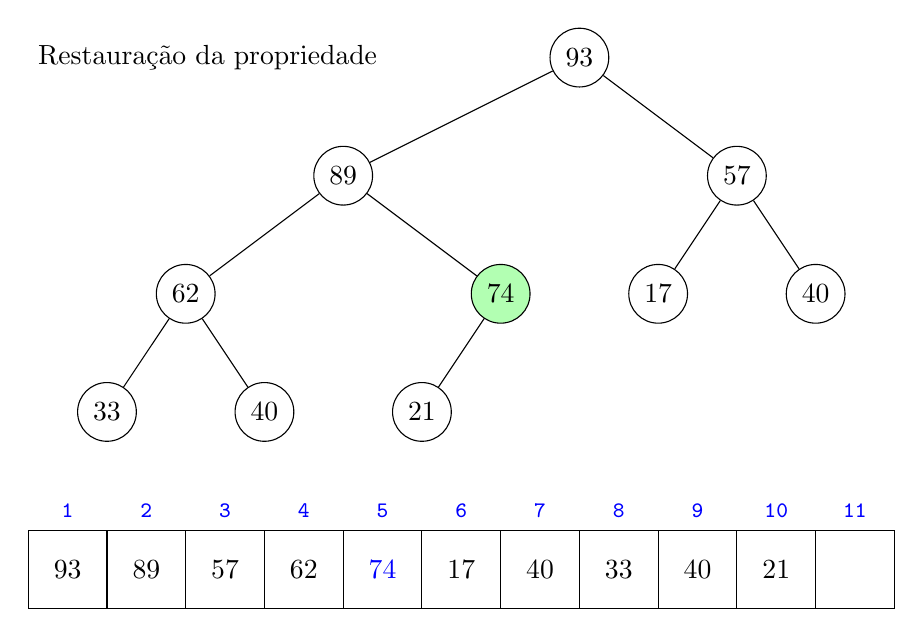
\begin{tikzpicture}
                \node[anchor=west] at (-1, 6) { Restauração da propriedade };
                \node[circle,draw] (A) at (6, 6) { 93 };
                \node[circle,draw] (B) at (3, 4.5) { \textcolor{black}{89} };
                \node[circle,draw] (C) at (8, 4.5) { 57 };
                \node[circle,draw] (D) at (1, 3) { 62 };
                \node[circle,draw,fill=green!30] (E) at (5, 3) { 74 };
                \node[circle,draw] (F) at (7, 3) { 17 };
                \node[circle,draw] (G) at (9, 3) { 40 };
                \node[circle,draw] (H) at (0, 1.5) { 33 };
                \node[circle,draw] (I) at (2, 1.5) { 40 };
                \node[circle,draw] (J) at (4, 1.5) { 21 };

                \draw (A) -- (B);
                \draw (A) -- (C);
                \draw (B) -- (D);
                \draw (B) -- (E);
                \draw (C) -- (F);
                \draw (C) -- (G);
                \draw (D) -- (H);
                \draw (D) -- (I);
                \draw (E) -- (J);

                \draw (-1, -1) grid (10, 0);

                \node[color=blue] at (-0.5, 0.25) { \footnotesize \texttt{\textbf{1}} };
                \node[color=blue] at (0.5, 0.25) { \footnotesize \texttt{\textbf{2}} };
                \node[color=blue] at (1.5, 0.25) { \footnotesize \texttt{\textbf{3}} };
                \node[color=blue] at (2.5, 0.25) { \footnotesize \texttt{\textbf{4}} };
                \node[color=blue] at (3.5, 0.25) { \footnotesize \texttt{\textbf{5}} };
                \node[color=blue] at (4.5, 0.25) { \footnotesize \texttt{\textbf{6}} };
                \node[color=blue] at (5.5, 0.25) { \footnotesize \texttt{\textbf{7}} };
                \node[color=blue] at (6.5, 0.25) { \footnotesize \texttt{\textbf{8}} };
                \node[color=blue] at (7.5, 0.25) { \footnotesize \texttt{\textbf{9}} };
                \node[color=blue] at (8.5, 0.25) { \footnotesize \texttt{\textbf{10}} };
                \node[color=blue] at (9.5, 0.25) { \footnotesize \texttt{\textbf{11}} };

                \node at (-0.5, -0.5) { \textcolor{black}{93} };
                \node at (0.5, -0.5) { \textcolor{black}{89} };
                \node at (1.5, -0.5) { 57 };
                \node at (2.5, -0.5) { 62 };
                \node at (3.5, -0.5) { \textcolor{blue}{74} };
                \node at (4.5, -0.5) { 17 };
                \node at (5.5, -0.5) { 40 };
                \node at (6.5, -0.5) { 33 };
                \node at (7.5, -0.5) { 40 };
                \node at (8.5, -0.5) { 21 };
        \end{tikzpicture}
    \end{figure}

\end{frame}

\begin{frame}[fragile]{Implementação da extração em \textit{heap} binária}
    \inputsnippet{cpp}{39}{59}{heap.cpp}
\end{frame}

\begin{frame}[fragile]{Implementação da extração em \textit{heap} binária}
    \inputsnippet{cpp}{60}{77}{heap.cpp}
\end{frame}
